\chapter{A cognitive approach to represent automotive scenes}%
\label{chap:a_cognitive_approach_to_represent_automotive_scenes}

We have seen in chapter ~\ref{chap:research_context}, especially in section ~\ref{subsec:knowledge_representation}, that, already today, there is a plethora of \acfp{ADAS} in intelligent vehicles. 
In future vehicles, the number of modules tackling different sub-tasks necessary to enable (semi-) autonomous driving and to interact with humans inside and outside the car will increase even more.
Given the complexity of the physical world and the recent success of \acp{DNN} in the diverse applications, a substantial amount of such modules could be data-driven with increasingly large neural networks under the surface.
In a worst case scenario, each of these systems will encapsulate its own representation of knowledge about the data it processes in complete separation from other, potentially related systems.
Typically, the representations used rely completely on numerical values and lack possibilities to be enriched or combined with symbol-like representations.
On the other hand, increasingly deep neural network architectures are not only hungry for data to generalize sufficiently enough from the examples they have been trained on, but also tend to require a substantial amount of computational resources.
Although this aspect is more severe for the training process, it becomes more important for mobile applications such as automated vehicles during the deployment phase.

In this thesis, we propose a novel representation for automotive scenes based on modern cognitive modeling techniques, namely the \ac{SPA}.
The \ac{SPA} is one particular example from a family of cognitive architectures commonly referred to as \acp{VSA} (see section ~\ref{subsec:vector_based_approaches} and chapter ~\ref{chap:introduction_to_vsas} for further details).
One of the key components of these cognitive architectures is to use high-dimensional vectors for representation.
This representational approach offers several desirable features.
High-dimensional vectors are one variant of distributed representations in the sense, that information is captured over all dimensions of the vector instead of one single number.
This aspect makes distributed representations more robust to noise in the sense, that a few noisy entries influence the overall information carried by the vector less compared to low-dimensional representations.
Furthermore, vector representations allow to encode both, symbol-like and numerical structures in a similar and unified way.
Additionally, the algebraic operations enable manipulation and combination of represented entities into structured representations.
One potential advantage of this approach is that the number of dimensions remains fixed independent of the number of entities combined through the architecture's algebraic operations.
Finally, vectors are a suitable representational substrate to be used in combination with neural networks.
On the one hand, vectors are a natural input to classic \acp{ANN}, but they also offer the possibility to be efficiently implement in \acp{SNN} using the principles of the \ac{NEF} (see \cite{Eliasmith2013}, but also section ~\ref{subsec:implementation_in_snns}).
Given an widespread implementation of the representations proposed here in combination with \acp{SNN} as algorithmic substrate within intelligent vehicles, the latter offers the potential to deploy such neural representations on dedicated neuromorphic hardware (cf.\ section ~\ref{sec:neuromorphic_HW}).
Although neuromorphic computing hardware as well as the corresponding neural algorithms are mainly used in academic research and often lack the technical maturity required by industrial applications, they show promise to be an energy-efficient option for future automated vehicles.

In this chapter, we introduce our proposed approach to encapsulate high-level information about automotive scenes in a high-dimensional vector representation.
In this context, high-level information refers to already preprocessed or even fused data about objects in the driving environment.
We analyze how different types of data could be encoded in such a representation and show possible variations and how they influence the final representation.
Thereby, we lay the basis for concrete application examples investigated in forthcoming chapters.

\begin{itemize}
	\item several driver assistance systems/sub-tasks of automated driving
	\subitem in the worst case different kind of knowledge representation for each
	\subitem this representation is usually not informative to the user

	\item machine learning/\ac{AI} (or data driven approaches in general) become increasingly important $\rightarrow$ unified system for knowledge representation necessary/helpful
	\item \aclp{VSA} offer the opportunity to combine advantages of symbolism and neural networks (through the principles of the \acf{NEF})
	\item automotive as a mobile application (with increasingly many ML/AI driven applications) demands for energy efficiency $\rightarrow$ \acp{VSA} can be applied on neuromorphic hardware
	\item outline scene representation in vector format. how is it currently realized? How could it develop/evolve if (more) sensors would natively support it.
	\item problem of how to encode numerical information (vector length vs trigonomical vs. unitary vector powers) for values of position, velocity etc.
	\item possibility to encode structure (first results from Robert's thesis)
\end{itemize}

\section{Vector representation of automotive scenes}
\subsection{What types of data to encode?}
\subsection{Structured representations}
\subsubsection{Limiting factors to structured representations}
\begin{figure}[t]
	\centering
	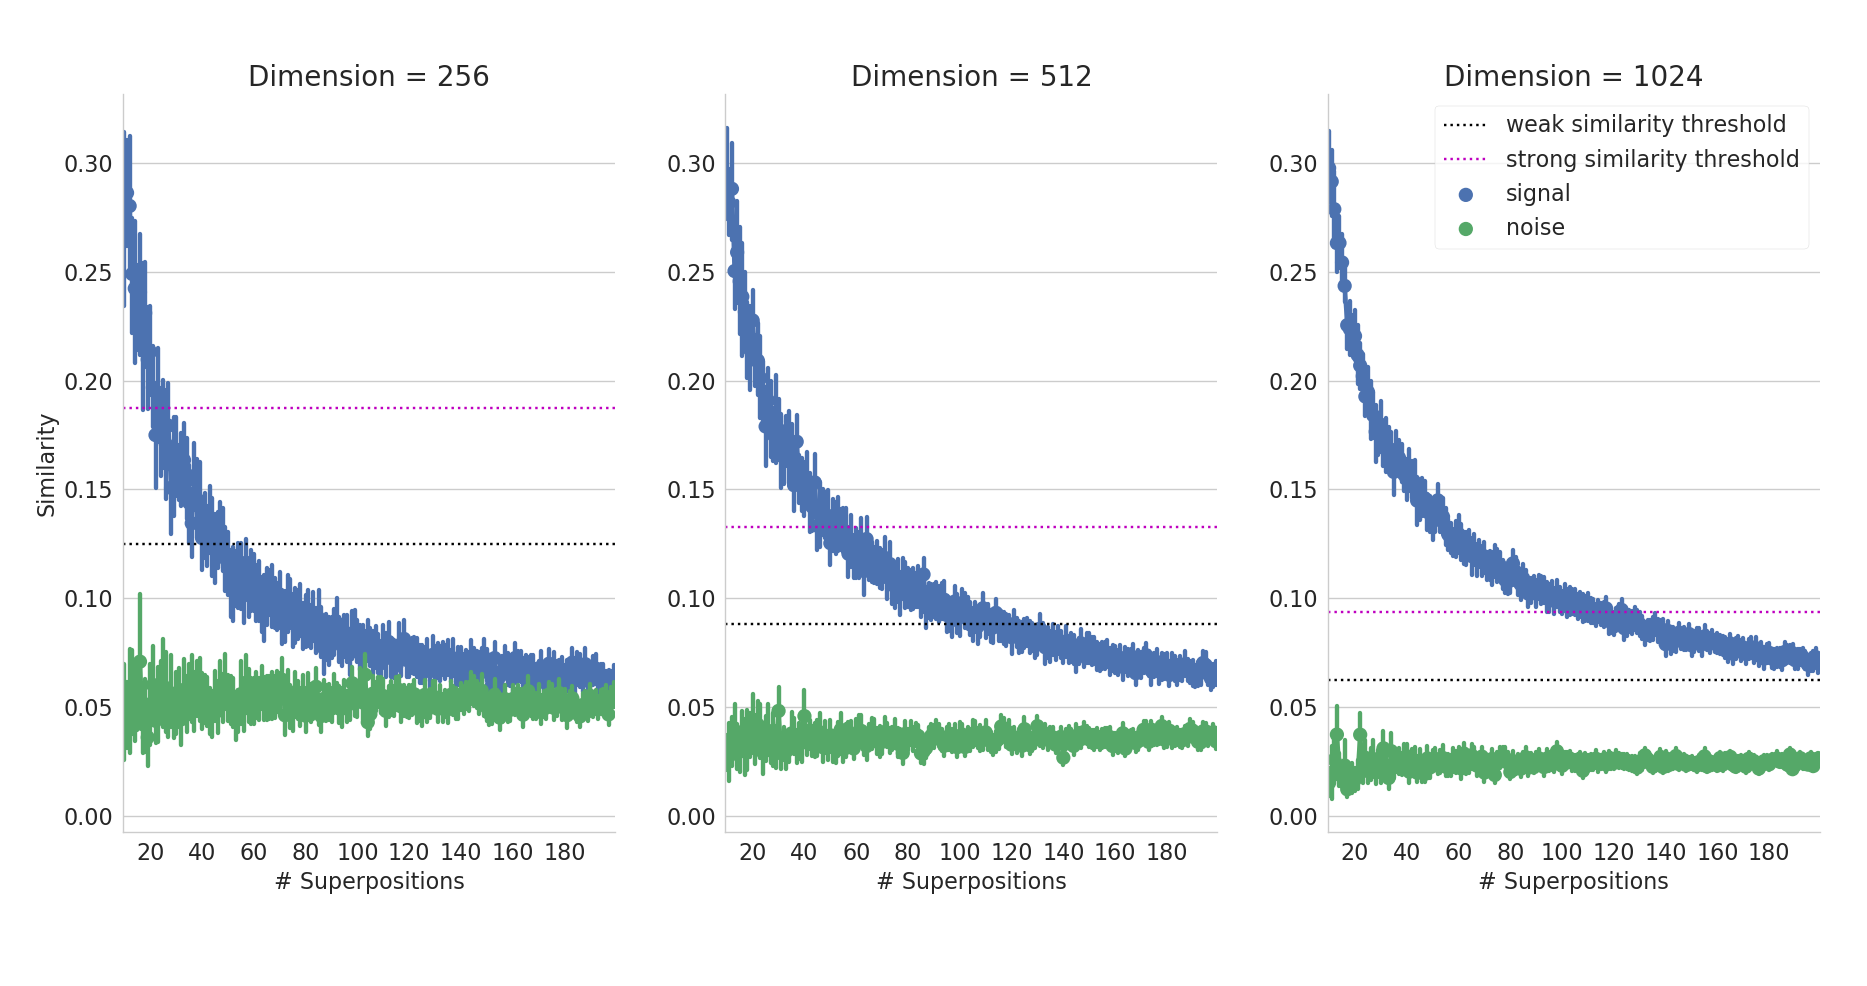
\includegraphics[width=0.95\textwidth]{imgs/spa_superposition_capacity.png}
	\caption{Superposition capacity.}
	\label{fig:spa_superposition_capacity}
\end{figure}

\section{Representational variations}
\subsection{Basic (random) vocabularies}
\subsection{Different vector representations for numerical values}
In this section, we investigate different approaches to map numerical information to semantic vectors.
Therefore, we will focus on
\subsubsection{Scalar multiplication encoding}
\subsubsection{Sine and Cosine encoding with different frequencies and offsets}
For vectorization of two-dimensional values, we use an encoding with sine and cosine functions with different spatial frequencies and offsets.
Therefore, we define the following helper functions
\[ \abb{f_{\left(m,i\right)}}{\mathbb{R}^2}{\mathbb{R}^4}{\left(x,y\right)}{\left(\cos\frac{m\cdot \pi + x}{i + 1}, \sin\frac{m\cdot \pi + x}{i + 1}, \cos\frac{m\cdot \pi + y}{i + 1}, \sin\frac{m\cdot \pi + y}{i + 1}\right)},
\]
\[
\abb{\psi_i}{\mathbb{R}^2}{\mathbb{R}^4}{\left(x,y\right)}{\left(f_{\left(0,i\right)}\left(x,y\right), f_{\left(\frac{1}{2},i\right)}\left(x,y\right), f_{\left(1,i\right)}\left(x,y\right), f_{\left(\frac{3}{2},i\right)}\left(x,y\right)\right)}
\]
and obtain the final vector representation of acceleration in $x$/$y$-direction via the function
\[
\abb{\lambda}{\mathbb{R}^2}{\mathbb{R}^D}{\left(x,y\right)}{\frac{1}{\sqrt{\frac{D}{2}}}\left(\psi_0\left(x,y\right), \cdots, \psi_{\frac{D}{16}-1}\left(x,y\right)\right).}
\]
This encoding $\lambda\left(a_x, a_y\right)$ leads to normalized, nonzero, similar vectors with information distributed over all elements (in contrast to a simple encoding like $\left(a_x, a_y, 0 \cdots, 0\right)$).
\subsubsection{Convolutive power encoding}
\subsection{Encoding visual and semantic structure}
